\documentclass{beamer}
\usepackage[utf8]{inputenc}
\usepackage[T1]{fontenc}
\usepackage[frenchb]{babel}
\usepackage{hyperref}
\usepackage{listings}
\usepackage{verbatim}

\title{Formation LaTeX - ouverture}
\date{\today}
\author{KI'019}

\usetheme{ki}

\begin{document}

\begin{frame}
    \titlepage
\end{frame}

\begin{frame}
    \frametitle{La vérité sur LaTeX}
    \begin{enumerate}
        \item<1-> IDE : Miktek, Texmaker
        \item<2-> Compilateur / éditeur : texlive / Kile, Vim, Emacs, Gedit, Notepad++     
        \item<3-> Tex, LaTeX, BibTeX, LuaLaTex, XeLaTeX...
    \end{enumerate}
\end{frame}

\begin{frame}[fragile]
    \frametitle{Les présentations}
    \begin{enumerate}
        \item<1-> le type beamer
        \item<2-> L'environement double colonne
        \begin{lstlisting}[language=TeX]
\begin{columns}
 \begin{column}[c]{6cm}
  \begin{itemize}
   \item Des dessins, des graphes...
    \url{http://www.texample.net/media/tikz/...}
  \end{itemize}
 \end{column}
 \begin{column}[c]{5cm}
  \includegraphics[width=5cm]{...pdf}
 \end{column}
\end{columns}
        \end{lstlisting}
    \end{enumerate}
\end{frame}

\begin{frame}
    \frametitle{Un éditeur d'image ?}
    \framesubtitle{Tikz et pgf}
 \begin{columns}
    \begin{column}[c]{6cm}
    \begin{itemize}
        \item<1-> Des dessins, des graphes...
        \url{http://www.texample.net/media/tikz/examples/PDF/phasor-diagram.pdf}
        \item<2-> Exportation géogébra
    \end{itemize}

    \end{column}
    \begin{column}[c]{5cm}
	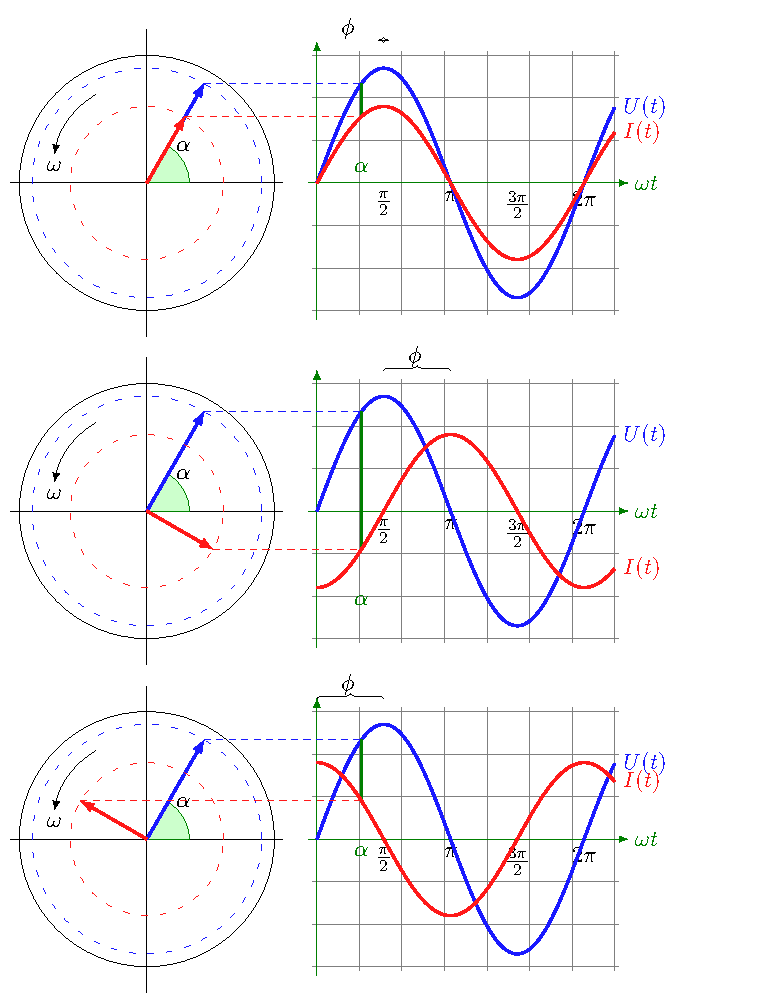
\includegraphics[width=5cm]{phasor-diagram.pdf}
    \end{column}
  \end{columns}
\end{frame}

\begin{frame}[fragile]
    \frametitle{Python avec LaTeX}
\begin{columns}
    \begin{column}[c]{7cm}
    \begin{itemize}
        \item<1-> LaTeX dans Matplotlib : r' '
        \begin{lstlisting}[language=TeX]
xtitle(r'Déformation \xi_x 
en fonction de \sigma_{xx}')
        \end{lstlisting}
        \item<2-> Changer la police, la taille...
        \url{https://matplotlib.org/users/usetex.html}
        \item<3-> LaTeX dans Jupyter, exporter un notebook en LaTeX
    \end{itemize}

    \end{column}
    \begin{column}[c]{4cm}
	
\includegraphics[width=4cm]{logo-ki.pdf}
    \end{column}
  \end{columns}
\end{frame}

\begin{frame}[fragile]
    \frametitle{Formatage des paragraphes}
     \begin{lstlisting}
\usepackage[a4paper, total={6in, 8in}]{geometry}
\usepackage[utf8]{inputenc}

\setlength{\parindent}{4em}
\setlength{\parskip}{1em}
\renewcommand{\baselinestretch}{2}      
     \end{lstlisting}
\end{frame}

\begin{frame}[fragile]
    \frametitle{Inclure du code non-formaté}
    \framesubtitle{listings}
       \begin{itemize}
       \item<1-> Inclure le module :
     \begin{lstlisting}
\usepackage{listings}      
     \end{lstlisting}
       \item<2-> Ecrire du code non-formaté dans le fichier tex :
\lstinputlisting{lstlisting.exemple}
       \item<3-> Inclure un fichier de code à côté :
     \begin{lstlisting}[language=TeX]
\lstinputlisting[language=Python, firstline=37, 
lastline=45]{source_filename.py}       
     \end{lstlisting}
       \end{itemize}
\end{frame}

\begin{frame}[fragile]
    \frametitle{Faire un lien}
    \begin{enumerate}
        \item<1-> Inclure le module :
        \begin{lstlisting}[language=TeX]
\usepackage{hyperref}
        \end{lstlisting}
        \item<2-> Faire des liens :
        \begin{lstlisting}[language=TeX]
\url{https://en.wikibooks.org/wiki/LaTeX}
\href{https://en.wikibooks.org}{Un lien}
        \end{lstlisting}
        \item<3-> Dans un beamer :
        \begin{lstlisting}[language=TeX]
\begin{frame}[fragile]
        \end{lstlisting}
        \item<4-| alert@1> \href{https://www.codecogs.com/latex/eqneditor.php}{Online code editor}
        \item<5-| alert@1> \href{https://fr.sharelatex.com/templates}{Templates} : bibliographie, livre, sujet d'examen, calendrier, CV, thèse, slides, article scientifique, template de supaero...
    \end{enumerate}
\end{frame}

\begin{frame}
    \frametitle{LaTeX fait-il du café ?}
    \begin{enumerate}
        \item<1-> LaTeX est turing-complet
        \item<2-> Créer des macros (donc des fonctions)        
        \item<3-> La suite de Fibonacci :\\
        \url{https://fr.sharelatex.com/blog/2012/04/24/latex-is-more-powerful-than-you-think.html}
        \item<4-> Un interpréteur de Basic
        \url{http://tug.org/TUGboat/Articles/tb11-3/tb29greene.pdf}
        \item<5-> Créer une classe, créer des paquets...
    \end{enumerate}
\end{frame}

\begin{frame}[fragile]
    \frametitle{Conseils et liens utiles}
    \begin{enumerate}
        \item<1-> Tester très souvent la compilation car la moindre '\}' oubliée donne une erreur incompréhensible car l'erreur est indiquée à la fin de l'environnement / page 
        \item<2-> mode mathématiques de LaTeX sans autocomplétion = folie
        \item<3-> Online code editor : \url{https://www.codecogs.com/latex/eqneditor.php}
        \item<4-> Templates : bibliographie, livre, sujet d'examen, calendrier, CV, thèse, slides, article scientifique, template de supaero...
        \url{https://fr.sharelatex.com/templates}
    \end{enumerate}
\end{frame}

\end{document}
